\documentclass[xcolor = {svgnames,x11names}]{beamer}

\mode<presentation> {
  \usetheme{Malmoe}
  % ou autre ...

  \setbeamercovered{transparent}
  % ou autre chose (il est également possible de supprimer cette ligne)
}


%\usepackage[english]{babel}
% or autre comme par exemple \usepackage[english]{babel}

%\usepackage[latin1]{inputenc}
% or autre

\usepackage{times}
%\usepackage[T1]{fontenc}
% Or autre. Notez que le codage et la fonte doivent être assortis. Si T1
% ne paraît pas très esthétique, essayer d'effacer la ligne contenant fontenc.

\usepackage{color}
\usepackage{tikz}
\usetikzlibrary{arrows,positioning}
\usepackage{algorithm}
\usepackage{algorithmic}
\usepackage{hyperref}
\usepackage{multimedia}
\usepackage{listings}
\usepackage[utf8]{inputenc}
\usepackage[frenchb]{babel}
\usepackage{aeguill}
\usepackage{import}

\newcommand\vect[1]{\textbf{#1}}
\newcommand\CS{{\cal C}}
\newcommand\rational{\mathbb{Q}}
\newcommand\real{\mathbb{R}}
\newcommand\Sone{\mathbb{S}^1}
\newcommand\conf{\textbf{q}}
\newcommand\x{\vect{x}}
\newcommand\y{\vect{y}}
\newcommand\z{\vect{z}}
\newcommand\WS{{\cal W}}
\newcommand\robot{{\cal R}}
\newcommand\body{{\cal B}}
\newcommand\obst{{\cal O}}
\newcommand\CSobst{\CS_{obst}}
\newcommand\CSfree{\CS_{free}}
\newcommand\sturm{\textbf{sturm}}
\newcommand\var{\textbf{n}_{chsgn}}
\newcommand\nor{\textbf{nr}}
\newcommand\signe{\textbf{signe}}
\newcommand\Kappa{{\cal K}}
\newcommand\calP{{\cal P}}
\newcommand\moment{\vect{M}}
\newcommand\resultante{\vect{R}}
\newcommand\f{\vect{f}}
\newcommand\vel{\vect{v}}
\newcommand\gravity{\vect{g}}
\newcommand\trans{\vect{t}}
\newcommand\rotation{R}
\newcommand\utheta{u_{\theta}}
\newcommand\cinematique{\mathcal{V}}
\newcommand\alcv{{\cal A}}
\newcommand\mloc{{\cal M}_{loc}}
\newcommand\control{\mathbf{u}}
\newcommand\crossprod[1]{\left[{#1}\right]_{\times}}
\newcommand\angularmomentum{\mathbf{L}}
\newcommand\length{\ell}
\newcommand\yaw{\mbox{yaw}}
\definecolor{grey}{rgb}{0.5,0.5,0.5}


\title {Motion planning}

\subtitle{}

\author[]
{Florent Lamiraux}

\institute[CNRS-LAAS] % (facultatif mais généralement nécessaire)
{
  CNRS-LAAS, Toulouse, France
}
\date[] % (facultatif, peut être une abréviation du nom de la conférence)
{}

\begin{document}

\lstset{
breakatwhitespace=true,
%language=C++,
%columns=fullflexible,
%keepspaces=true,
breaklines=true
tabsize=3, 
%showstringspaces=false,
%extendedchars=true
}

\begin{frame}
  \titlepage
\end{frame}

%\input{intro}
\begin{frame}{Motion planning}
  \tableofcontents[currentsection,currentsubsection]
  % Vous pouvez, si vous le souhaiter ajouter l'option [pausesections]
\end{frame}

%\section {Introduction}
%
%  Definition
%
\begin {frame} {Context}
  \centerline {
    \parbox {3cm} {
      Industrial robots
      \vskip .2cm
      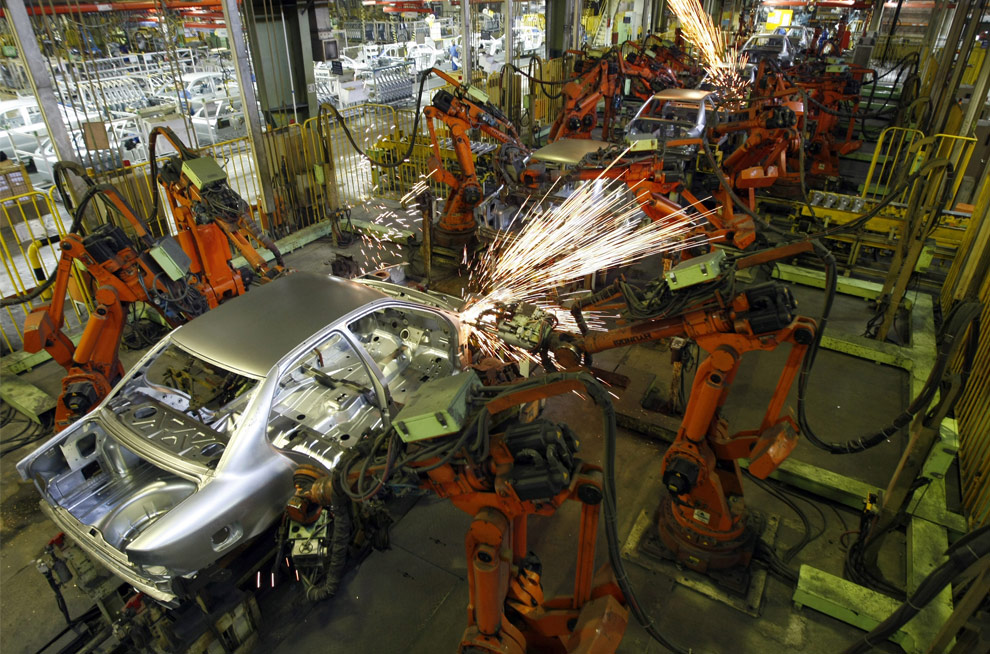
\includegraphics [height=2cm] {pictures/robot_welding_iran.jpg}
    }
    \hspace*{.05\linewidth}
    \parbox {3cm} {
      aerial robots
      \vskip .2cm
      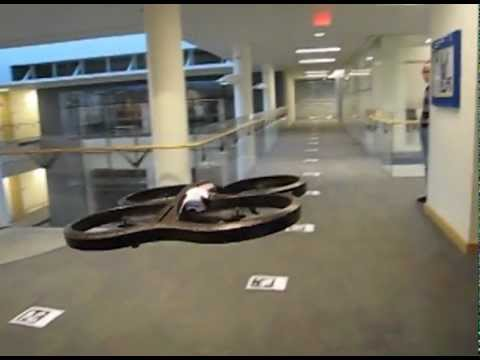
\includegraphics [height=2cm] {pictures/indoor-uav.jpg}
    }
    \hspace*{.05\linewidth}
    \parbox {3cm} {
      autonomous vehicles
      \vskip .2cm
      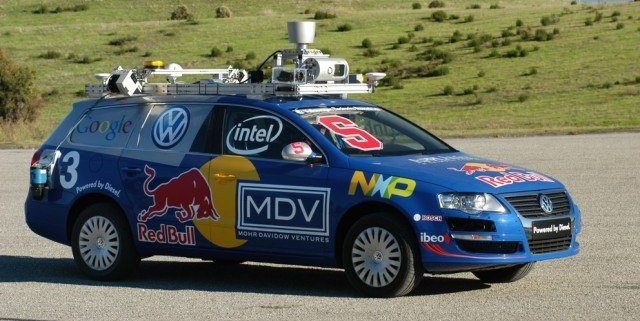
\includegraphics [height=2cm] {pictures/Google-robot-car.jpg}
    }
  }
  \vskip 1cm
  \pause
  Mobile autonomous system
  \begin{itemize}
    \item moving in an environment cluttered with obstacles
    \item subject to kinematic or dynamic constraints
  \end{itemize}
  \pause
  Motion planning~: automatically computing a feasible trajectory between two configurations.
\end {frame}

%\section {Définitions}

%
%  Robot
%

\begin{frame} {Robot}
  \centerline {
    \parbox{.66\linewidth} {
      Set of rigid bodies $\body_0,\cdots\body_m$, linked to one another by \textit{joints}.
      \vskip .5cm
      \centerline {
        \def\svgwidth {.5\linewidth}
        {\tiny
          \graphicspath{{./figures/}}
          \input {figures/kinematic-chain.pdf_tex}
        }
      }
      \vskip .5cm
      Joint~: parameterized rigid-body transformation between two frames (in SE(3)).
    }
    \parbox {.33\linewidth} {
      \centerline {
        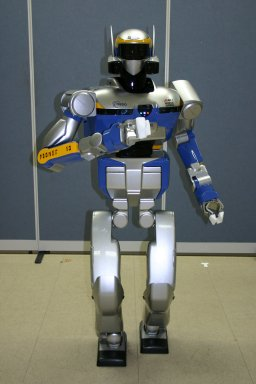
\includegraphics[width=\linewidth]{figures/hrp2.jpg}
      }
    }
  }
\end{frame}

%
%  Déplacement rigide
%

\begin {frame} {Rigid body transformation}
  Definitions
  \begin {itemize}
  \item SO(3)~: group of 3 by 3 rotation matrices.
   $$R\in SO(3) \Leftrightarrow R^TR = I_3\ \mbox{and}\ \det(R)=1$$
  \item SE(3)~: group of rigid body tranformations
    \begin{eqnarray*}
      T\in SE(3) \Leftrightarrow && \exists t\in\real^3, \exists R\in SO(3)\\
      && \forall x\in\real^3\ T(x) = Rx + t
    \end{eqnarray*}
    We denote $T = T_{(R,t)}$.
  \end{itemize}
\end{frame}

%
%  Articulation
%
\begin {frame} {Joint}
  A joint is represented by a mapping from a sub-manifold of $\real^p$ in SE(3),
  where $p\geq 1$ is an integer.\\
  Examples~:\\
  \centerline {
    \parbox {.5\linewidth} {
      \begin {itemize}
      \item Translation T1~:
        \begin{eqnarray*}
          \real & \rightarrow & SE(3) \\
          t & \rightarrow & T_{(I_3, (t\ 0\ 0))}
        \end{eqnarray*}
      \end {itemize}
      \vskip .5cm
    }
    \parbox {.49\linewidth} {translation along x}
  }
\end {frame}

%
%  Articulation
%
\begin {frame} {Joint}
  A joint is represented by a mapping from a sub-manifold of $\real^p$ in SE(3),
  where $p\geq 1$ is an integer.\\
  Examples~:\\
  \centerline {
    \parbox {.5\linewidth} {
      \begin {itemize}
      \item Translation T3~:
        \begin{eqnarray*}
          \real^3 & \rightarrow & SE(3) \\
          t & \rightarrow & T_{(I_3, t)}
        \end{eqnarray*}
      \end {itemize}
      \vskip .5cm
    }
    \parbox {.49\linewidth} {translation}
  }
\end {frame}

%
%  Articulation
%
\begin {frame} {Joint}
  A joint is represented by a mapping from a sub-manifold of $\real^p$ in SE(3),
  where $p\geq 1$ is an integer.\\
  Examples~:\\
  \centerline {
    \parbox {.5\linewidth} {
      \begin {itemize}
      \item Rotation R1~:
        \begin{eqnarray*}
          \real & \rightarrow & SE(3) \\
          t & \rightarrow & T_{(R, 0)}
        \end{eqnarray*}
      \end {itemize}
      \vskip .5cm
    }
    \parbox {.49\linewidth} {
      $$ R=\left(\begin{array}{ccc}\cos t & -\sin t & 0 \\ \sin t & \cos t & 0 \\ 0&0&1\end{array}\right)$$
    }
  }
\end {frame}

%
%  Articulation
%
\begin {frame} {Joint}
  A joint is represented by a mapping from a sub-manifold of $\real^p$ in SE(3),
  where $p\geq 1$ is an integer.\\
  Examples~:\\
  \centerline {
    \parbox {.5\linewidth} {
      \begin {itemize}
      \item Rotation R3~:
        \begin{eqnarray*}
          \real^4 & \rightarrow & SE(3) \\
          t & \rightarrow & T_{(R, 0)}
        \end{eqnarray*}
      \end {itemize}
      \vskip .5cm
    }
    \parbox {.49\linewidth} {
      {\tiny
        $$
          \|t\| = 1
          $$
          $$\begin{array}{c}R=\\
          \left(\begin{array}{ccc}1 - 2(t_2^2 + t_3^2) & 2t_2t_1 - 2t_3t_0 & 2t_3t_1 + 2t_2t_0\\ 2t_2t_1 + 2t_3t_0 & 1 - 2(t_1^2 + t_3^2) & 2t_3t_2 - 2t_1t_0\\ 2t_3t_1 - 2t_2t_0 & 2t_3t_2 + 2t_1t_0 & 1 - 2(t_1^2 + t_2^2)\end{array}\right)\end{array}$$
          $$t_0 + t_1 i + t_2 j + t_3 k\ \mbox{is a quaternion.}$$
      }
    }
  }
\end {frame}

%
%  Quaternion
%
\begin {frame} {Quaternions}
  \centerline {
    \parbox {.75\linewidth} {
      Non-commutative field isomorphic to $\real^4$, spanned by three elements
      $i, j, k$ that satisfy the following relations~:
      $$i^2 = j^2 = k^2 = ijk = -1$$
      \pause
      from which we immediately deduce
      $$ ij=k,\ jk=i,\ ki=j$$
    }
    \parbox {.24\linewidth} {
      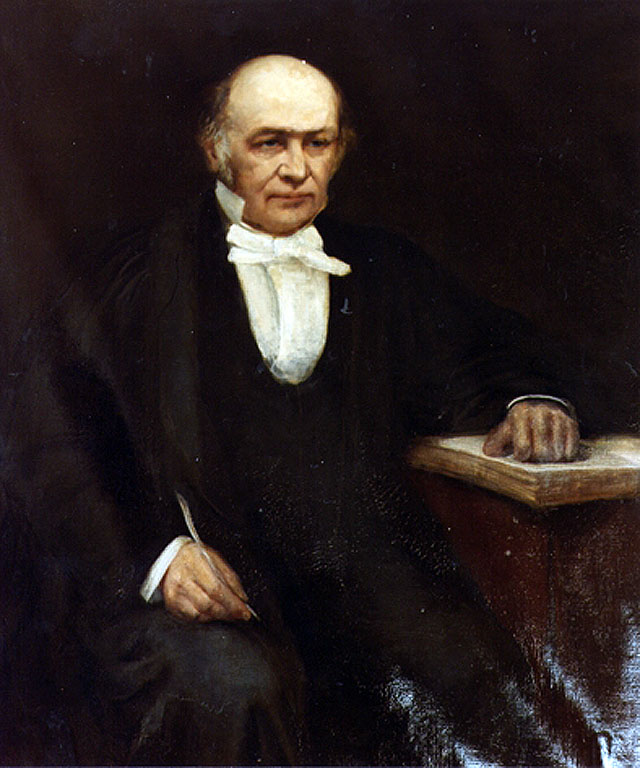
\includegraphics [width=\linewidth] {pictures/William_Rowan_Hamilton_painting.jpg}\\
      \centerline {Hamilton (1843)}
    }
  }
\end {frame}

%
%  Quaternions unitaires et rotations
%
\begin {frame} {Unit Quaternions and rotations}
  Let $q=q_0 + q_1 i + q_2 j + q_3 k$ be a unit quaternion:
  $$q_0^2 + q_3^2 + q_2^2 + q_3^2 = 1$$
  \pause
  $\forall x = (x_0, x_1, x_2)\in\real^3$, let $u=x_0i + x_1 j + x_2 k$
  $$
  q\,.\,u\,.\,q^* = y_0 i + y_1 j + y_2 k
  $$
  where $q^*=q_0 - q_1 i - q_2 j - q_3 k$ is the conjugate of $q$.\\
  \pause
  $y = (y_0, y_1, y_2)$ is the image of $x$ by the rotation of matrix
  $$
  \left(\begin{array}{ccc}1 - 2(q_2^2 + q_3^2) & 2q_2q_1 - 2q_3q_0 & 2q_3q_1 + 2q_2q_0\\ 2q_2q_1 + 2q_3q_0 & 1 - 2(q_1^2 + q_3^2) & 2q_3q_2 - 2q_1q_0\\ 2q_3q_1 - 2q_2q_0 & 2q_3q_2 + 2q_1q_0 & 1 - 2(q_1^2 + q_2^2)\end{array}\right)
  $$
\end{frame}

%
%  Quaternions unitaires et rotations
%
\begin {frame} {Unit Quaternions and rotations}
  \begin{itemize}
    \item Notice that $q$ and $-q$ represent the same rotation
    \item $SO(3)$ is isomorphic to $Sp(1)/\{\pm 1\}$, the half-sphere of
      $\real^4$.
  \end{itemize}
\end{frame}

%
%  Configuration d'un robot
%
\begin {frame} {Configuration of a robot}
  \centerline {
    \parbox{.66\linewidth} {
      The configuration $\conf$ of a robot is represented by the concatenation
      of the parameters of each joint.
      \vskip .5cm
      \centerline {
        \def\svgwidth {.5\linewidth}
        {\tiny
        \graphicspath{{./figures/}}
        \input {figures/kinematic-chain.pdf_tex}
        }
      }
    }
    \parbox {.33\linewidth} {
      \centerline {
        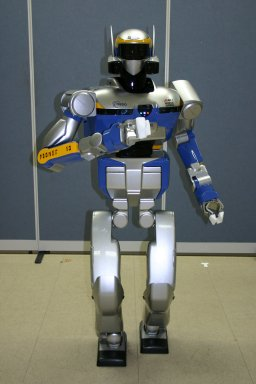
\includegraphics[width=\linewidth]{figures/hrp2.jpg}
      }
    }
  }
\end {frame}

%
%  Cinématique directe
%
\begin {frame} {Forward kinematics}
  \centerline {
    \parbox{.66\linewidth} {
      Computation of the position of each joint in the global frame
      $$
      M_i (\conf) = M_{parent (i)} (\conf)\ M_{i/parent}\ T_i (\conf)
      $$
      \centerline {
        \def\svgwidth {\linewidth}
        {\tiny
        \graphicspath{{./figures/}}
        \input {figures/forward-kinematics.pdf_tex}
        }
      }
    }
    \parbox {.33\linewidth} {
      \centerline {
        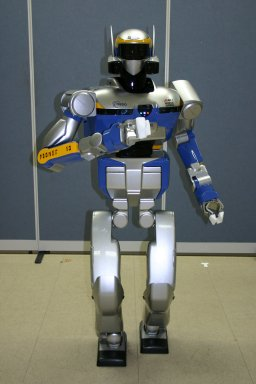
\includegraphics[width=\linewidth]{figures/hrp2.jpg}
      }
    }
  }
\end{frame}

%
%  Obstacle
%

\begin{frame} {Definitions}

\begin{itemize}
\item Workspace: $\WS=\real^2$ or $\real^3$: space in which the robot evolves
\pause
\item Obstacle in workspace: compact subset of $\WS$, denoted by $\obst$.
\pause
\item Configuration space: $\CS$.
\pause
\item Position in configuration $\conf$ of a point $M\in\body_i$:
  $\x_i(M,\conf)$.
\pause
\item Obstacle in the configuration space:
\begin{eqnarray*}
\CSobst&=\{\conf\in\CS,&\exists i\in\{1,\cdots,m\},\ \exists M\in\body_i,\ \x_i(M,\conf)\in\obst\ \mbox{or}\\
&&\exists i,j\in\{1,\cdots,m\},\ \exists M_i\in\body_i,\ \exists M_j\in\body_j,\\
&&\x_i(M_i,\conf)=x_j(M_j,\conf)\}
\end{eqnarray*}
\pause
\item Free configuration space: $\CSfree = \CS\setminus\CSobst$.
\end{itemize}
\end{frame}

%
%  Motion
%

\begin{frame} {Motion}

\begin{itemize}
\item Configuration space:
  \begin{itemize}
  \item differential manifold
  \end{itemize}
  \pause
\item Motion:
  \begin{itemize}
  \item continuous function from $[0,1]$ to $\CS$.
  \end{itemize}
  \pause
\item Collision-free motion:
  \begin{itemize}
  \item continuous function from $[0,1]$ to $\CSfree$.
  \end{itemize}
\end{itemize}
\end{frame}

%\section {Random methods}

%
%  random methods
%

\begin{frame} {Random methods}
  \begin{itemize}
  \item In the early 1990's, random methods started being developed
    \pause
  \item Principle
    \begin{itemize}
    \item shoot random configurations
      \pause
    \item test whether they are in collision
      \pause
    \item build a graph (roadmap)  the nodes of which are free configurations
      \pause
    \item  and the edges of which are collision-free linear interpolations
    \end{itemize}
  \end{itemize}
\end{frame}

%
%  La méthode du réseau aléatoire
%

\begin{frame} {Probabilistic roadmap (PRM) 1994}
\centerline {
  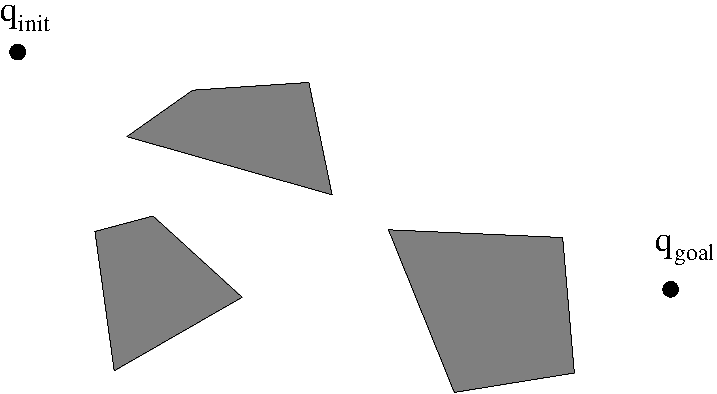
\includegraphics[width=.8\linewidth]{figures/PRM1.pdf}
}
\end{frame}

\begin{frame} {Probabilistic roadmap (PRM) 1994}
\centerline {
  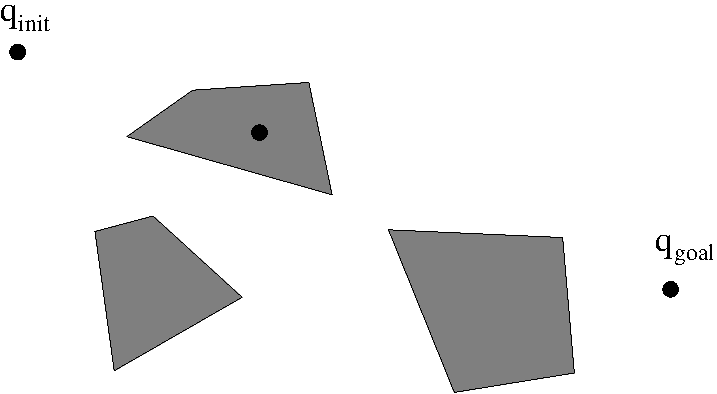
\includegraphics[width=.8\linewidth]{figures/PRM2.pdf}
}
\end{frame}

\begin{frame} {Probabilistic roadmap (PRM) 1994}
\centerline {
  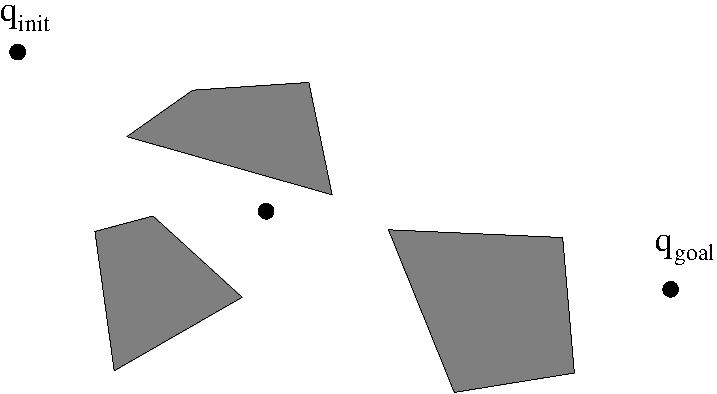
\includegraphics[width=.8\linewidth]{figures/PRM3.pdf}
}
\end{frame}

\begin{frame} {Probabilistic roadmap (PRM) 1994}
\centerline {
  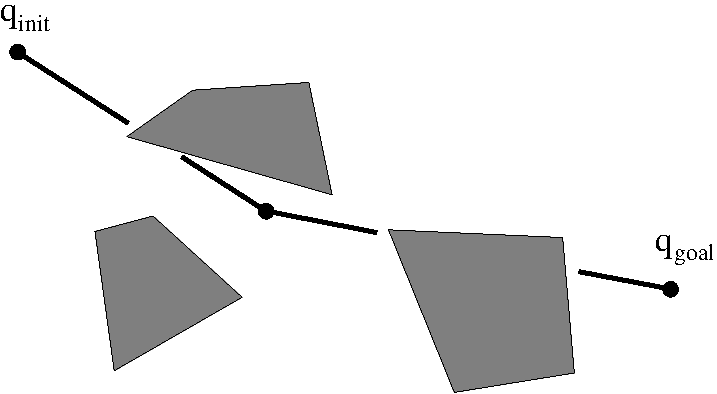
\includegraphics[width=.8\linewidth]{figures/PRM4.pdf}
}
\end{frame}

\begin{frame} {Probabilistic roadmap (PRM) 1994}
\centerline {
  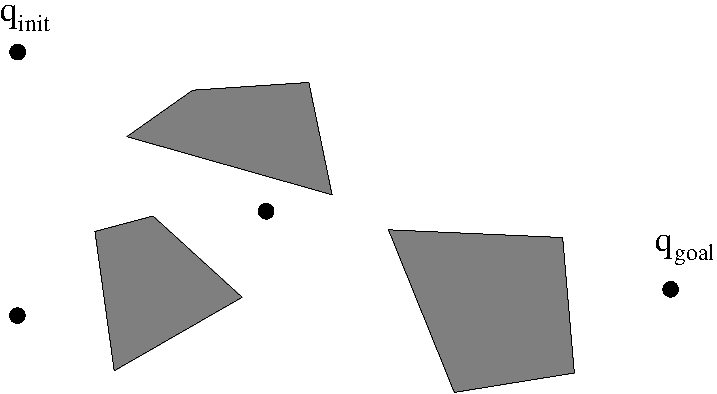
\includegraphics[width=.8\linewidth]{figures/PRM5.pdf}
}
\end{frame}

\begin{frame} {Probabilistic roadmap (PRM) 1994}
\centerline {
  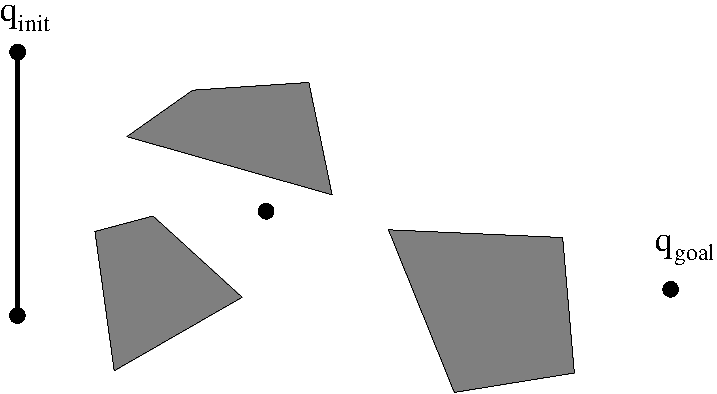
\includegraphics[width=.8\linewidth]{figures/PRM6.pdf}
}
\end{frame}

\begin{frame} {Probabilistic roadmap (PRM) 1994}
\centerline {
  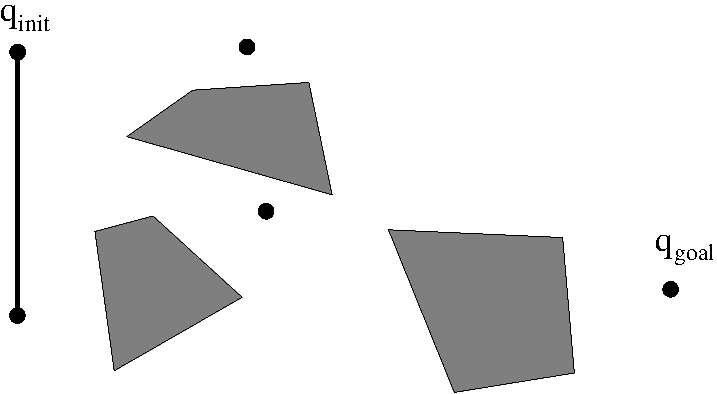
\includegraphics[width=.8\linewidth]{figures/PRM7.pdf}
}
\end{frame}

\begin{frame} {Probabilistic roadmap (PRM) 1994}
\centerline {
  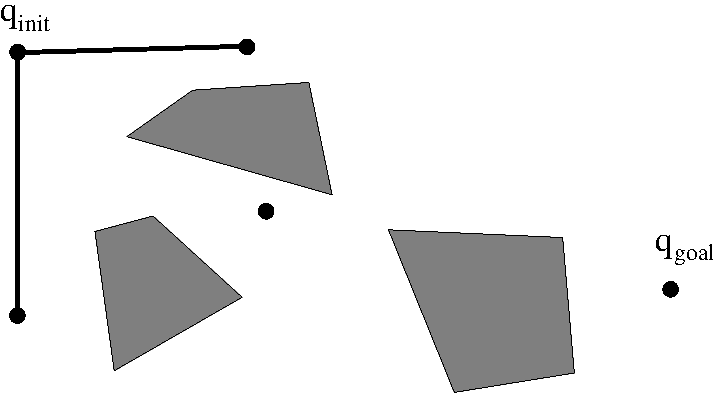
\includegraphics[width=.8\linewidth]{figures/PRM8.pdf}
}
\end{frame}

\begin{frame} {Probabilistic roadmap (PRM) 1994}
\centerline {
  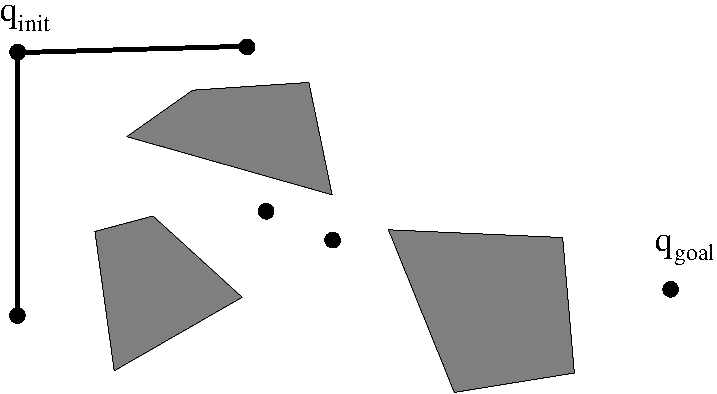
\includegraphics[width=.8\linewidth]{figures/PRM9.pdf}
}
\end{frame}

\begin{frame} {Probabilistic roadmap (PRM) 1994}
\centerline {
  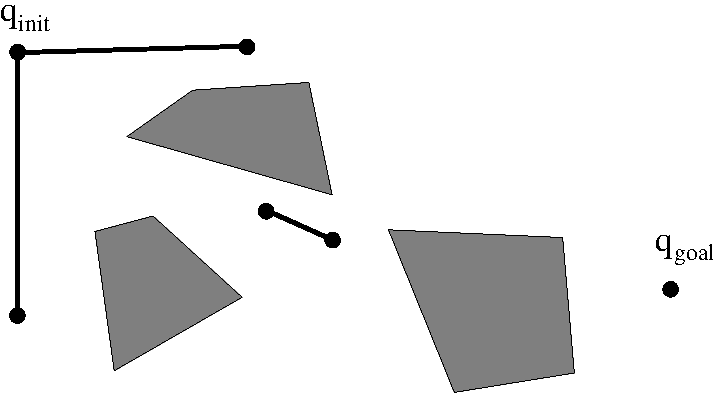
\includegraphics[width=.8\linewidth]{figures/PRM10.pdf}
}
\end{frame}

\begin{frame} {Probabilistic roadmap (PRM) 1994}
\centerline {
  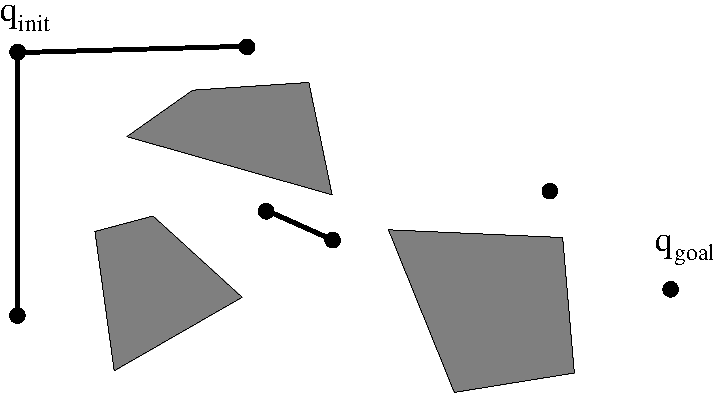
\includegraphics[width=.8\linewidth]{figures/PRM11.pdf}
}
\end{frame}

\begin{frame} {Probabilistic roadmap (PRM) 1994}
\centerline {
  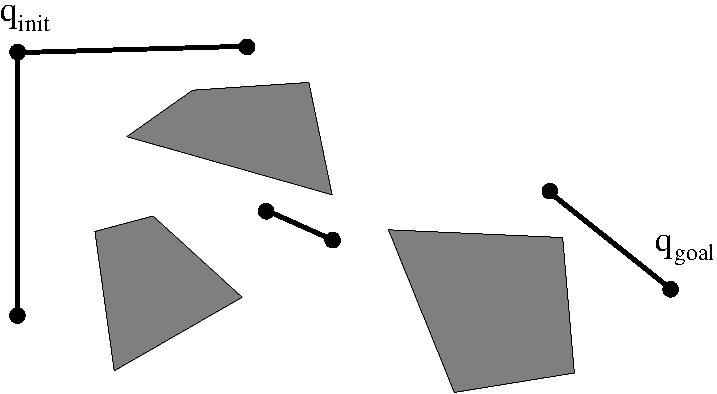
\includegraphics[width=.8\linewidth]{figures/PRM12.pdf}
}
\end{frame}

\begin{frame} {Probabilistic roadmap (PRM) 1994}
\centerline {
  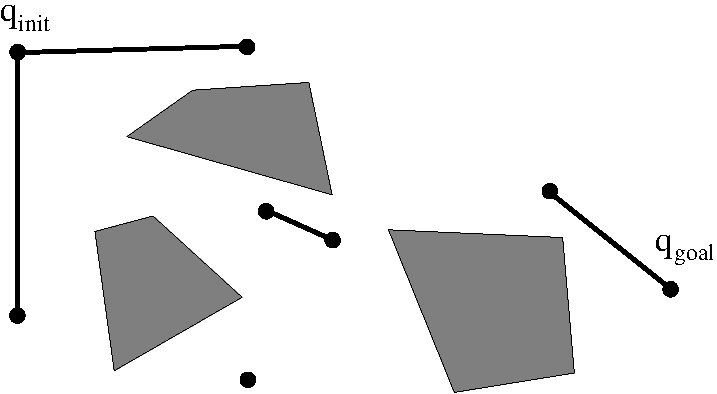
\includegraphics[width=.8\linewidth]{figures/PRM13.pdf}
}
\end{frame}

\begin{frame} {Probabilistic roadmap (PRM) 1994}
\centerline {
  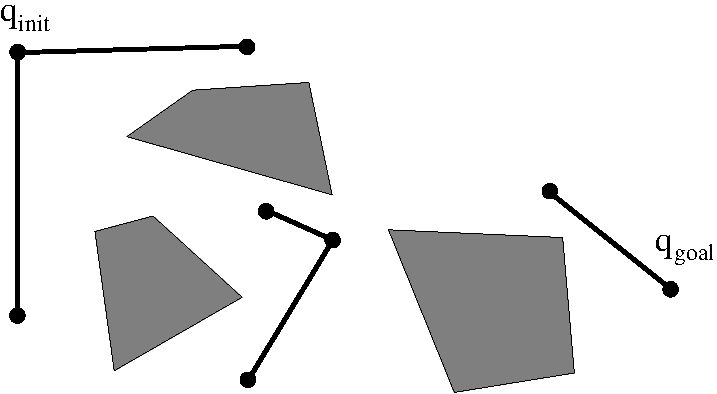
\includegraphics[width=.8\linewidth]{figures/PRM14.pdf}
}
\end{frame}

\begin{frame} {Probabilistic roadmap (PRM) 1994}
\centerline {
  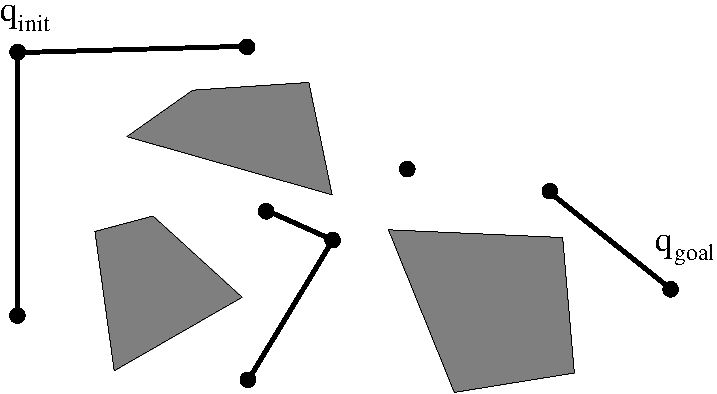
\includegraphics[width=.8\linewidth]{figures/PRM15.pdf}
}
\end{frame}

\begin{frame} {Probabilistic roadmap (PRM) 1994}
\centerline {
  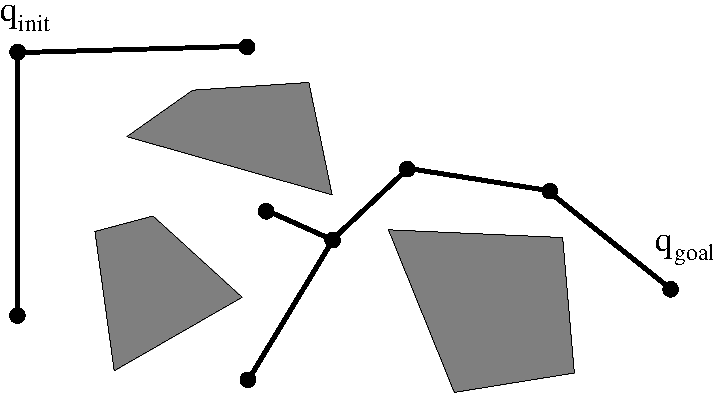
\includegraphics[width=.8\linewidth]{figures/PRM16.pdf}
}
\end{frame}

\begin{frame} {Probabilistic roadmap (PRM) 1994}
\centerline {
  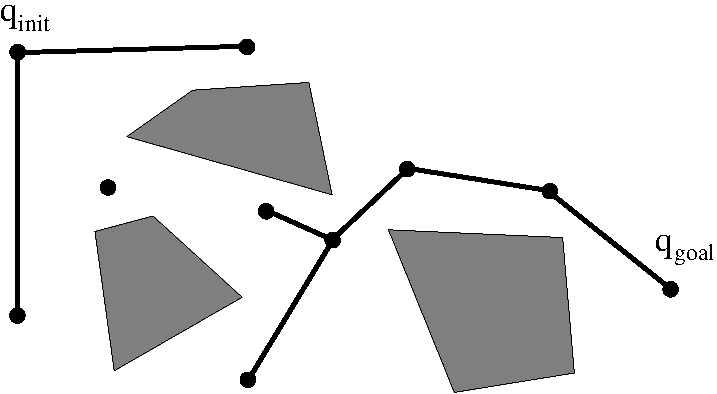
\includegraphics[width=.8\linewidth]{figures/PRM17.pdf}
}
\end{frame}

\begin{frame} {Probabilistic roadmap (PRM) 1994}
\centerline {
  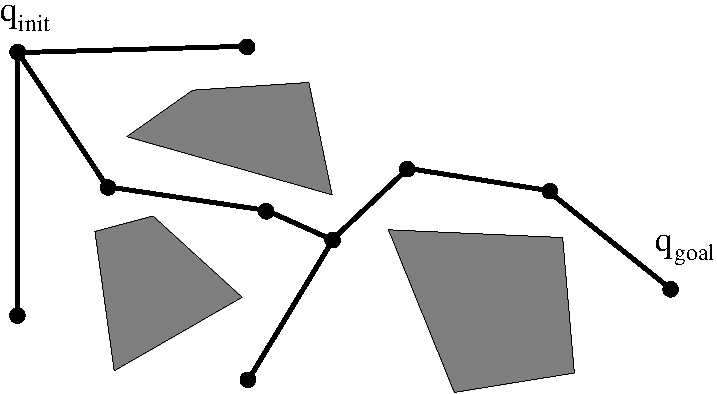
\includegraphics[width=.8\linewidth]{figures/PRM18.pdf}
}
\end{frame}

\begin{frame} {Probabilistic roadmap (PRM)}
  \begin{itemize}
  \item A lot of useless nodes are created,
    \begin{itemize}
    \item this increases the cost to connect new nodes to the existing roadmap
    \end{itemize}
  \item Improvement: visibility-based PRM
    \begin{itemize}
    \item Only \textit{interesting} nodes are kept.
    \end{itemize}
  \end{itemize}
\end{frame}


%
%  Visibility-based probabilistic roadmap
%
\begin{frame} {Visibility-based probabilistic roadmap (Visi-PRM) 1999}
\centerline {
  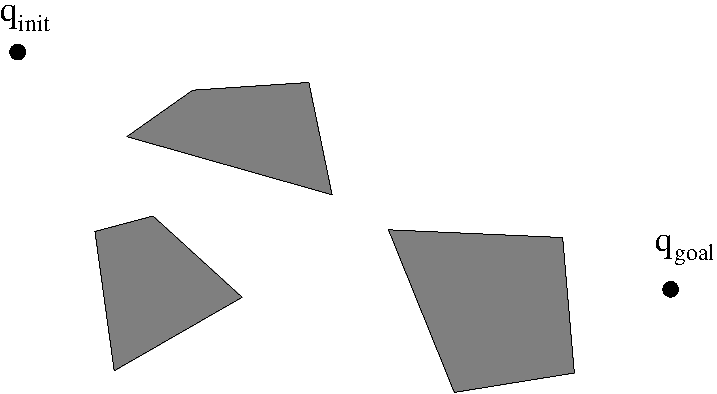
\includegraphics[width=.8\linewidth]{figures/VPRM1.pdf}
}
\end{frame}

\begin{frame} {Visibility-based probabilistic roadmap (Visi-PRM) 1999}
\centerline {
  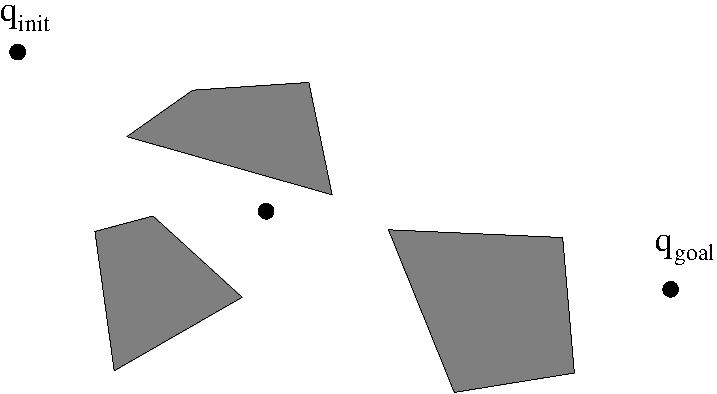
\includegraphics[width=.8\linewidth]{figures/VPRM2.pdf}
}
\end{frame}

\begin{frame} {Visibility-based probabilistic roadmap (Visi-PRM) 1999}
\centerline {
  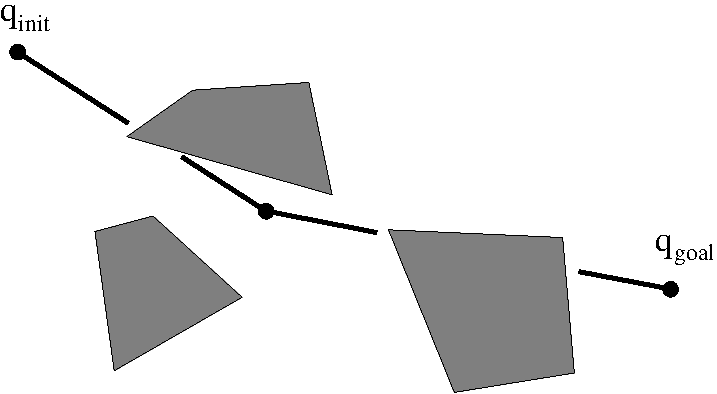
\includegraphics[width=.8\linewidth]{figures/VPRM3.pdf}
}
\end{frame}

\begin{frame} {Visibility-based probabilistic roadmap (Visi-PRM) 1999}
\centerline {
  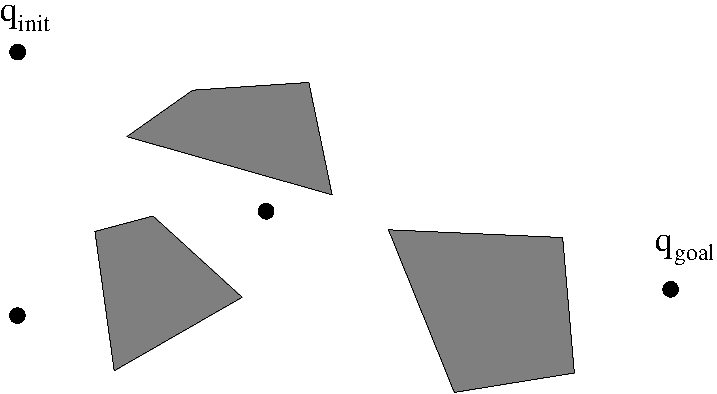
\includegraphics[width=.8\linewidth]{figures/VPRM4.pdf}
}
\end{frame}

\begin{frame} {Visibility-based probabilistic roadmap (Visi-PRM) 1999}
\centerline {
  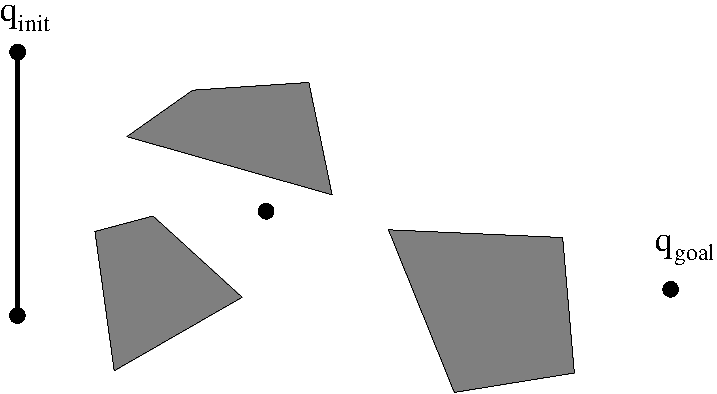
\includegraphics[width=.8\linewidth]{figures/VPRM5.pdf}
}
\end{frame}

\begin{frame} {Visibility-based probabilistic roadmap (Visi-PRM) 1999}
\centerline {
  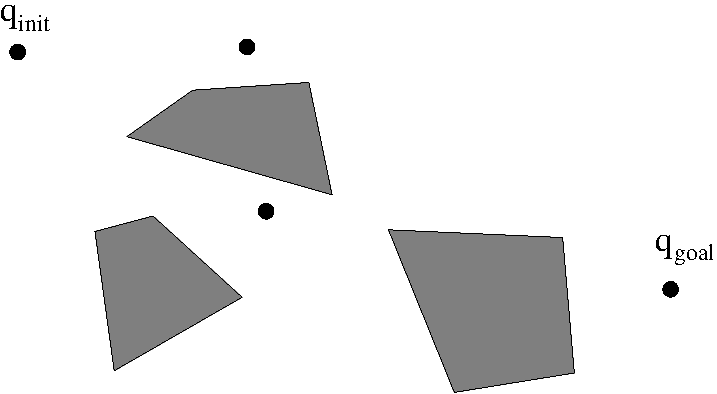
\includegraphics[width=.8\linewidth]{figures/VPRM6.pdf}
}
\end{frame}

\begin{frame} {Visibility-based probabilistic roadmap (Visi-PRM) 1999}
\centerline {
  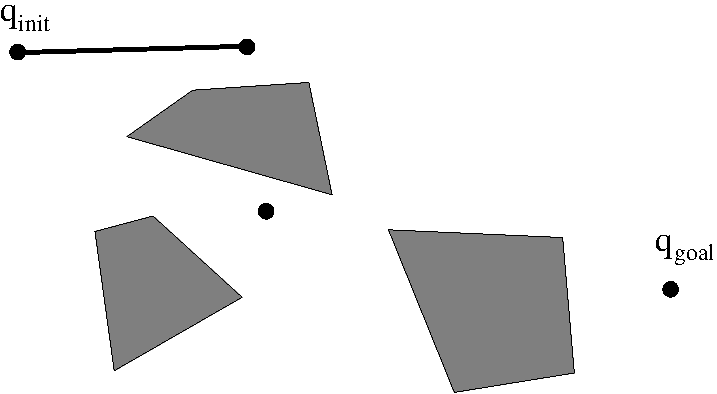
\includegraphics[width=.8\linewidth]{figures/VPRM7.pdf}
}
\end{frame}

\begin{frame} {Visibility-based probabilistic roadmap (Visi-PRM) 1999}
\centerline {
  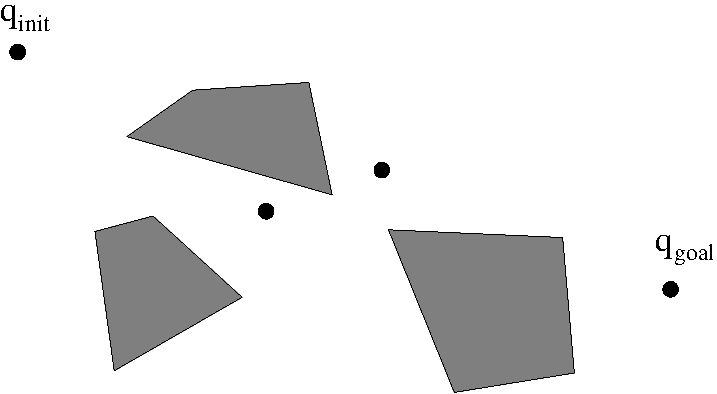
\includegraphics[width=.8\linewidth]{figures/VPRM8.pdf}
}
\end{frame}

\begin{frame} {Visibility-based probabilistic roadmap (Visi-PRM) 1999}
\centerline {
  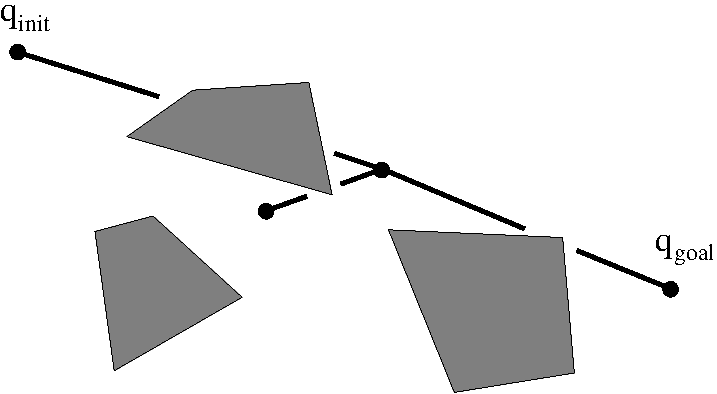
\includegraphics[width=.8\linewidth]{figures/VPRM9.pdf}
}
\end{frame}

\begin{frame} {Visibility-based probabilistic roadmap (Visi-PRM) 1999}
\centerline {
  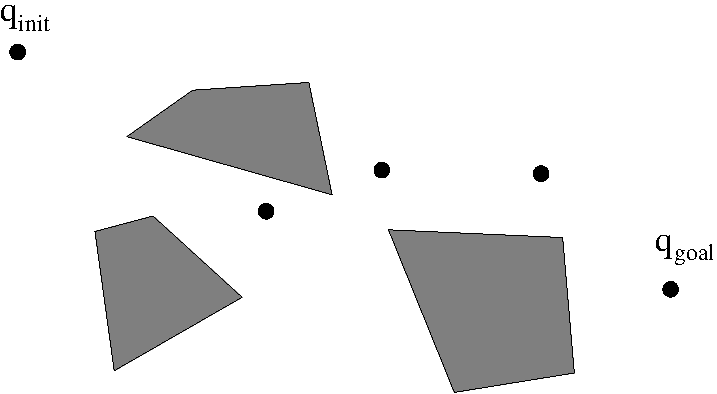
\includegraphics[width=.8\linewidth]{figures/VPRM10.pdf}
}
\end{frame}

\begin{frame} {Visibility-based probabilistic roadmap (Visi-PRM) 1999}
\centerline {
  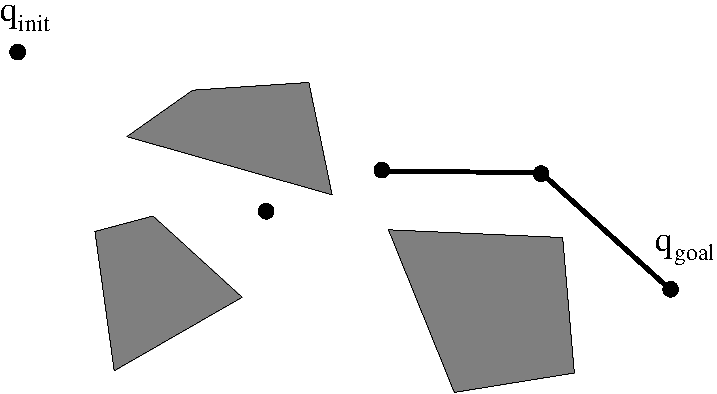
\includegraphics[width=.8\linewidth]{figures/VPRM11.pdf}
}
\end{frame}

\begin{frame} {Visibility-based probabilistic roadmap (Visi-PRM) 1999}
\centerline {
  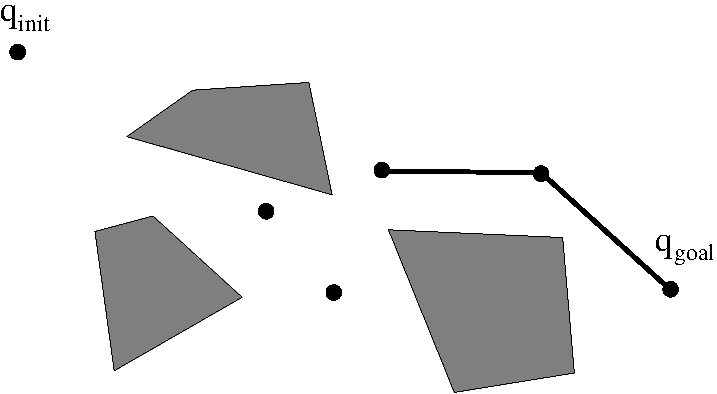
\includegraphics[width=.8\linewidth]{figures/VPRM12.pdf}
}
\end{frame}

\begin{frame} {Visibility-based probabilistic roadmap (Visi-PRM) 1999}
\centerline {
  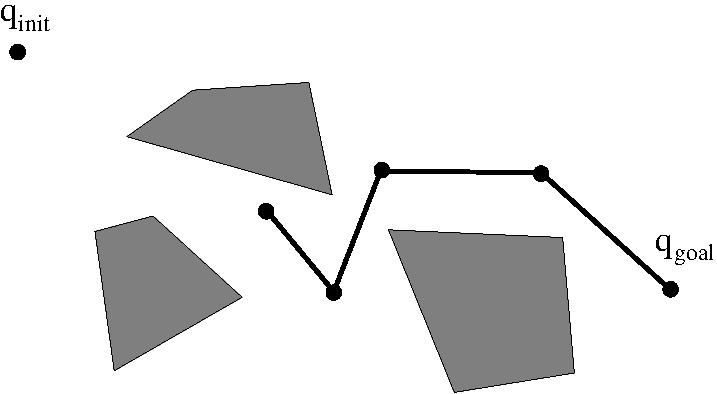
\includegraphics[width=.8\linewidth]{figures/VPRM13.pdf}
}
\end{frame}

\begin{frame} {Visibility-based probabilistic roadmap (Visi-PRM) 1999}
\centerline {
  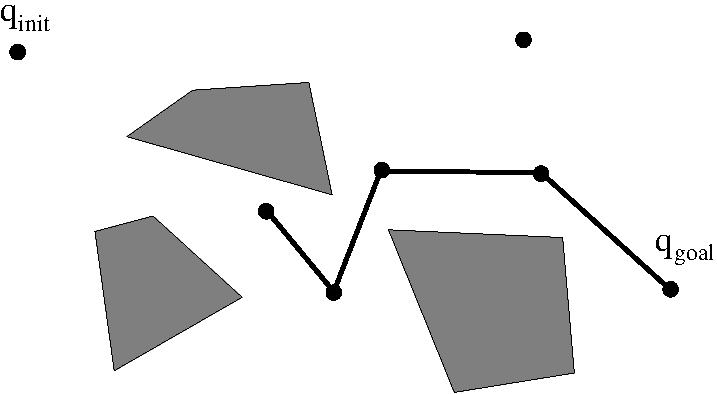
\includegraphics[width=.8\linewidth]{figures/VPRM14.pdf}
}
\end{frame}

\begin{frame} {Visibility-based probabilistic roadmap (Visi-PRM) 1999}
\centerline {
  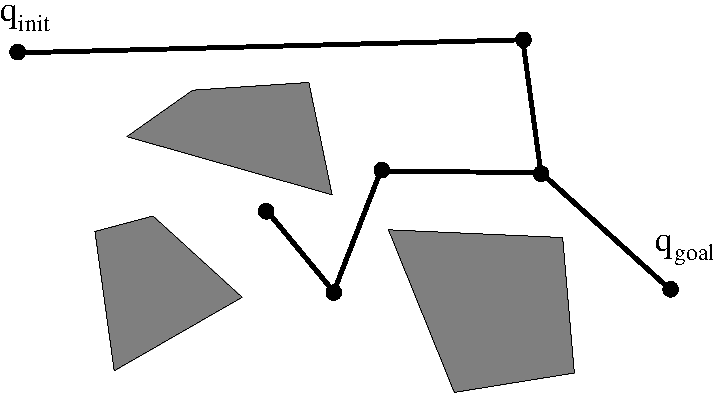
\includegraphics[width=.8\linewidth]{figures/VPRM15.pdf}
}
\end{frame}

%
%  La méthode des arbres aléatoires d'exploration rapide.
%

\begin{frame} {Rapidly exploring Random Tree (RRT) 2000}
\centerline {
  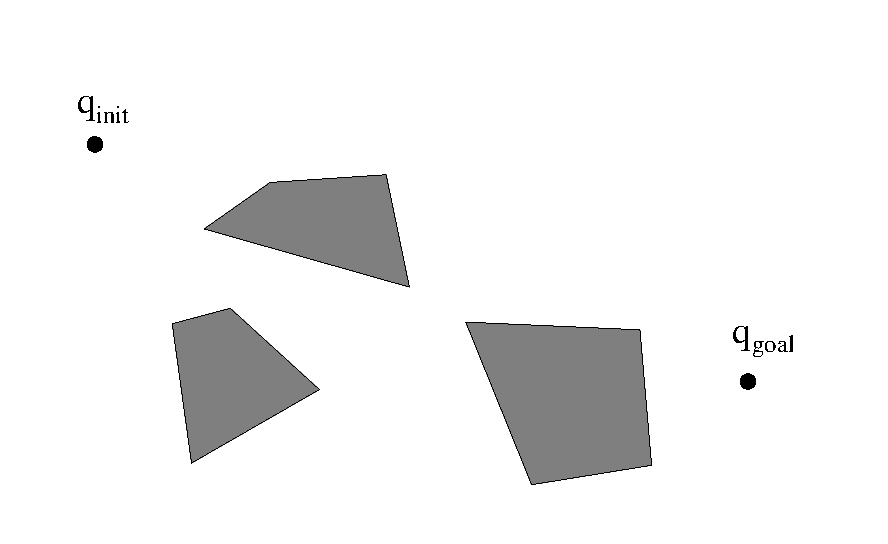
\includegraphics[width=.8\linewidth]{figures/RRT1.pdf}
}
\end{frame}

\begin{frame} {Rapidly exploring Random Tree (RRT) 2000}
\centerline {
  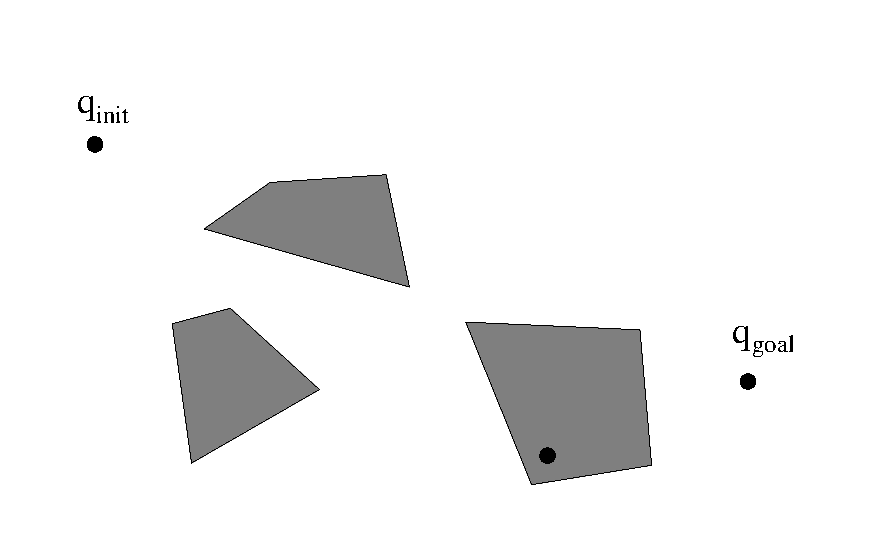
\includegraphics[width=.8\linewidth]{figures/RRT2.pdf}
}
\end{frame}

\begin{frame} {Rapidly exploring Random Tree (RRT) 2000}
\centerline {
  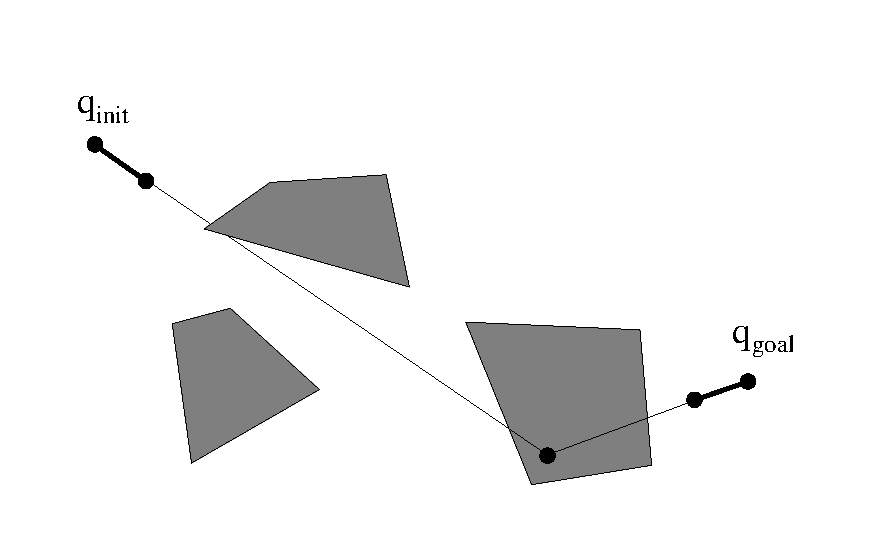
\includegraphics[width=.8\linewidth]{figures/RRT3.pdf}
}
\end{frame}

\begin{frame} {Rapidly exploring Random Tree (RRT) 2000}
\centerline {
  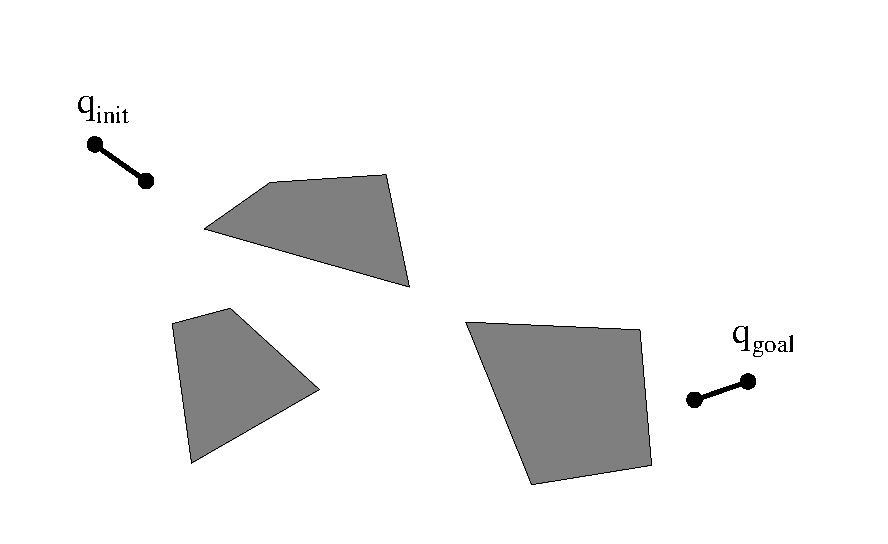
\includegraphics[width=.8\linewidth]{figures/RRT4.pdf}
}
\end{frame}

\begin{frame} {Rapidly exploring Random Tree (RRT) 2000}
\centerline {
  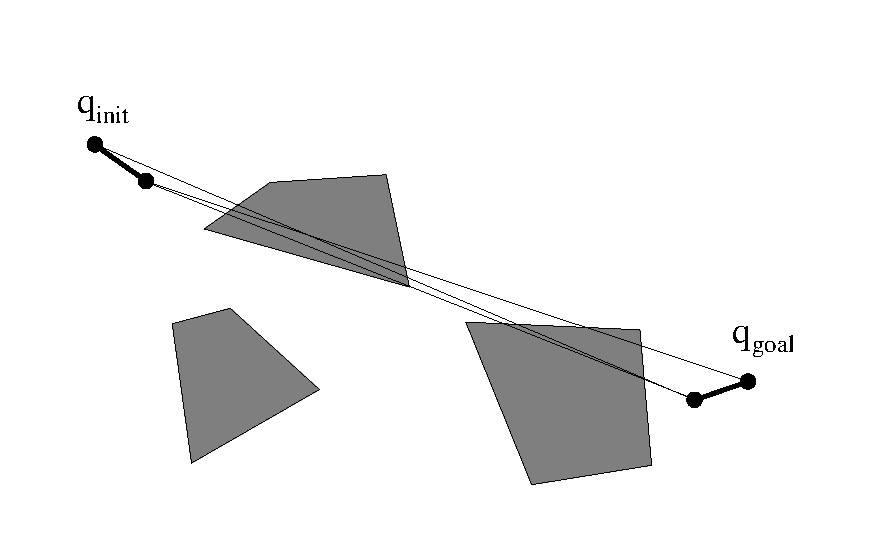
\includegraphics[width=.8\linewidth]{figures/RRT5.pdf}
}
\end{frame}

\begin{frame} {Rapidly exploring Random Tree (RRT) 2000}
\centerline {
  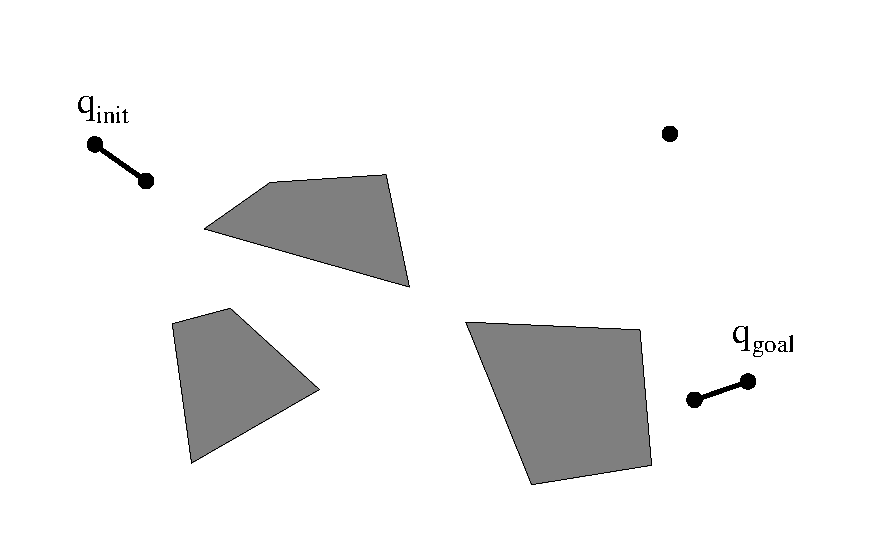
\includegraphics[width=.8\linewidth]{figures/RRT6.pdf}
}
\end{frame}

\begin{frame} {Rapidly exploring Random Tree (RRT) 2000}
\centerline {
  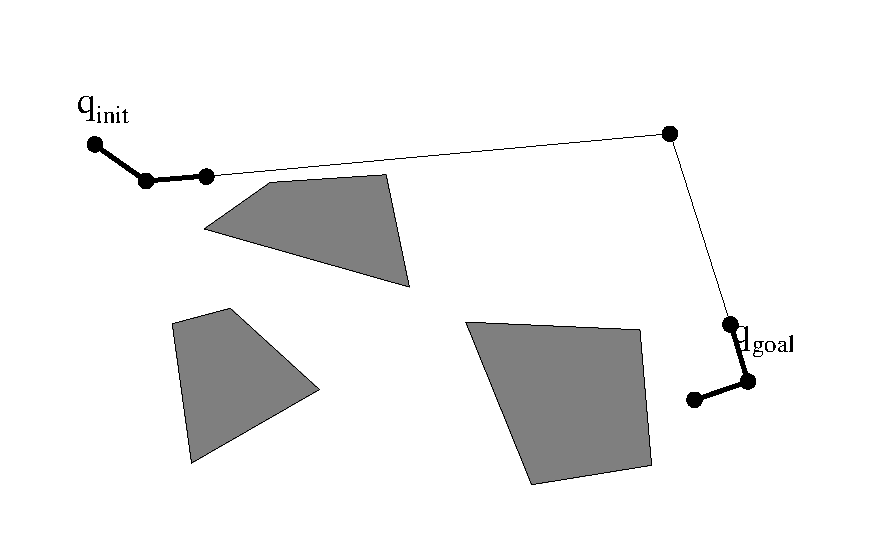
\includegraphics[width=.8\linewidth]{figures/RRT7.pdf}
}
\end{frame}

\begin{frame} {Rapidly exploring Random Tree (RRT) 2000}
\centerline {
  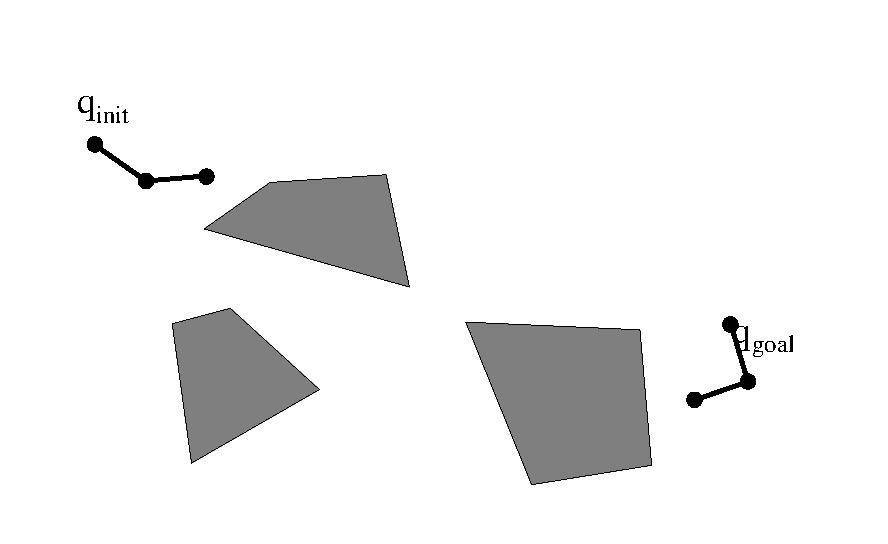
\includegraphics[width=.8\linewidth]{figures/RRT8.pdf}
}
\end{frame}

\begin{frame} {Rapidly exploring Random Tree (RRT) 2000}
\centerline {
  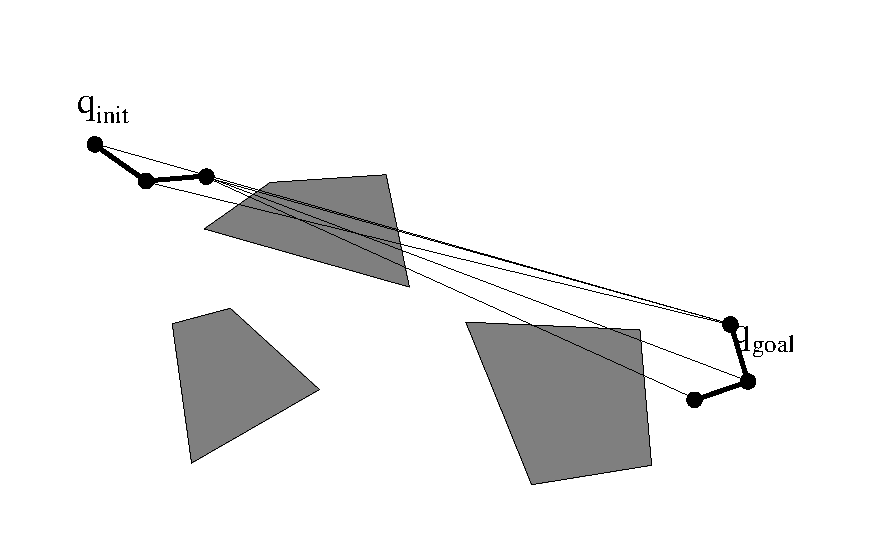
\includegraphics[width=.8\linewidth]{figures/RRT9.pdf}
}
\end{frame}

\begin{frame} {Rapidly exploring Random Tree (RRT) 2000}
\centerline {
  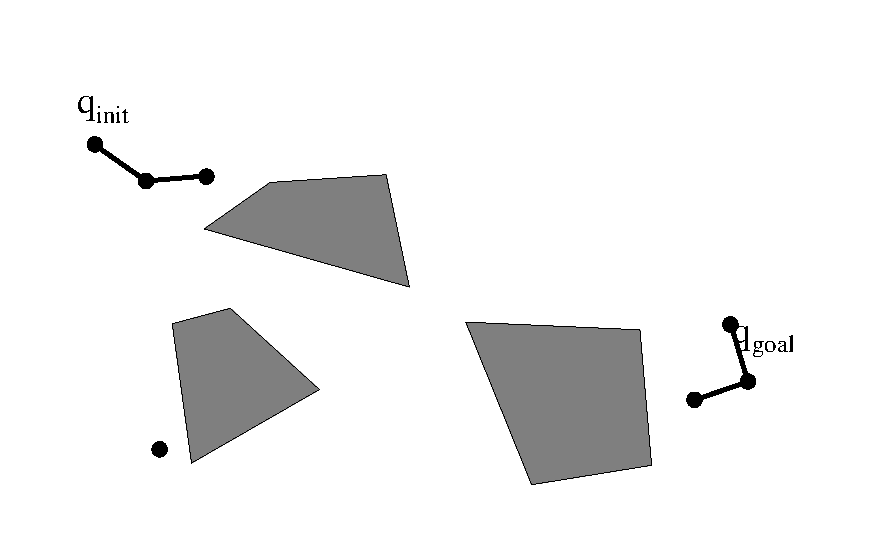
\includegraphics[width=.8\linewidth]{figures/RRT10.pdf}
}
\end{frame}

\begin{frame} {Rapidly exploring Random Tree (RRT) 2000}
\centerline {
  \includegraphics[width=.8\linewidth]{figures/RRT11.pdf}
}
\end{frame}

\begin{frame} {Rapidly exploring Random Tree (RRT) 2000}
\centerline {
  \includegraphics[width=.8\linewidth]{figures/RRT12.pdf}
}
\end{frame}

\begin{frame} {Rapidly exploring Random Tree (RRT) 2000}
\centerline {
  \includegraphics[width=.8\linewidth]{figures/RRT13.pdf}
}
\end{frame}

\begin{frame} {Rapidly exploring Random Tree (RRT) 2000}
\centerline {
  \includegraphics[width=.8\linewidth]{figures/RRT14.pdf}
}
\end{frame}

\begin{frame} {Rapidly exploring Random Tree (RRT) 2000}
\centerline {
  \includegraphics[width=.8\linewidth]{figures/RRT15.pdf}
}
\end{frame}

\begin{frame} {Rapidly exploring Random Tree (RRT) 2000}
\centerline {
  \includegraphics[width=.8\linewidth]{figures/RRT16.pdf}
}
\end{frame}

\begin{frame} {Rapidly exploring Random Tree (RRT) 2000}
\centerline {
  \includegraphics[width=.8\linewidth]{figures/RRT17.pdf}
}
\end{frame}

\begin{frame} {Rapidly exploring Random Tree (RRT) 2000}
\centerline {
  \includegraphics[width=.8\linewidth]{figures/RRT18.pdf}
}
\end{frame}

\begin{frame} {Rapidly exploring Random Tree (RRT) 2000}
\centerline {
  \includegraphics[width=.8\linewidth]{figures/RRT19.pdf}
}
\end{frame}

\begin{frame} {Rapidly exploring Random Tree (RRT) 2000}
\centerline {
  \includegraphics[width=.8\linewidth]{figures/RRT20.pdf}
}
\end{frame}

%
% random methods
%

\begin{frame} {Random methods}
  \begin{itemize}
  \item Pros:
    \begin{itemize}
    \item no explicit computation of the free configuration space,
    \item easy to implement,
    \item robust.
    \end{itemize}
    \pause
  \item Cons:
    \begin{itemize}
    \item no completeness property, only probabilistic completeness,
    \item difficult to find narrow passages.
    \end{itemize}
    \pause
  \item Requested operators~:
    \begin{itemize}
    \item Collision tests
      \begin{itemize}
      \item for configurations (static),
      \item for paths (dynamic)
      \end{itemize}
    \end{itemize}
  \end{itemize}
\end{frame}

%\section {Collision tests}

%
%  Collision tests
%
\begin{frame} {Collision tests}
  \begin{itemize}
  \item for configurations
    \begin{itemize}
    \item problem: given
      \begin{itemize}
      \item two rigid sets of triangles,
      \item the relative position of one set with respect to the other set,
      \end{itemize}
      determine whether the intersection between the sets is empty, or compute
      the distance between the sets.
    \end{itemize}
  \end{itemize}
\end{frame}

%
%  Hierarchy of bounding volumes
%
\begin{frame} {Hierarchy of bounding volumes}
  \begin{itemize}
  \item Binary trees of bounding volumes such that
    \begin{itemize}
    \item each node contains two children,
    \item leaves are the triangles
    \end{itemize}
  \end{itemize}
  \centerline {
    \includegraphics[width=.8\linewidth]{figures/bvh1.pdf}
  }
\end{frame}

\begin{frame} {Hierarchy of bounding volumes}
  \begin{itemize}
  \item Binary trees of bounding volumes such that
    \begin{itemize}
    \item each node contains two children,
    \item leaves are the triangles
    \end{itemize}
  \end{itemize}
  \centerline {
    \includegraphics[width=.8\linewidth]{figures/bvh2.pdf}
  }
\end{frame}

\begin{frame} {Hierarchy of bounding volumes}
  \begin{itemize}
  \item Binary trees of bounding volumes such that
    \begin{itemize}
    \item each node contains two children,
    \item leaves are the triangles
    \end{itemize}
  \end{itemize}
  \centerline {
    \includegraphics[width=.8\linewidth]{figures/bvh3.pdf}
  }
\end{frame}

\begin{frame} {Hierarchy of bounding volumes}
  \begin{itemize}
  \item Binary trees of bounding volumes such that
    \begin{itemize}
    \item each node contains two children,
    \item leaves are the triangles
    \end{itemize}
  \end{itemize}
  \centerline {
    \includegraphics[width=.8\linewidth]{figures/bvh4.pdf}
  }
\end{frame}

\begin{frame} {Hierarchy of bounding volumes}
  \begin{itemize}
  \item Binary trees of bounding volumes such that
    \begin{itemize}
    \item each node contains two children,
    \item leaves are the triangles
    \end{itemize}
  \end{itemize}
  \centerline {
    \includegraphics[width=.8\linewidth]{figures/bvh5.pdf}
  }
\end{frame}

\begin{frame} {Hierarchy of bounding volumes}
  \begin{itemize}
  \item Binary trees of bounding volumes such that
    \begin{itemize}
    \item each node contains two children,
    \item leaves are the triangles
    \end{itemize}
  \end{itemize}
  \centerline {
    \includegraphics[width=.8\linewidth]{figures/bvh6.pdf}
  }
\end{frame}

\begin{frame} {Hierarchy of bounding volumes}
  \begin{itemize}
  \item Binary trees of bounding volumes such that
    \begin{itemize}
    \item each node contains two children,
    \item leaves are the triangles
    \end{itemize}
  \end{itemize}
  \centerline {
    \includegraphics[width=.8\linewidth]{figures/bvh7.pdf}
  }
\end{frame}

\begin{frame} {Hierarchy of bounding volumes}
  \begin{itemize}
  \item Binary trees of bounding volumes such that
    \begin{itemize}
    \item each node contains two children,
    \item leaves are the triangles
    \end{itemize}
  \end{itemize}
  \centerline {
    \includegraphics[width=.8\linewidth]{figures/bvh8.pdf}
  }
\end{frame}

\begin{frame} {Hierarchy of bounding volumes}
  \begin{itemize}
  \item Binary trees of bounding volumes such that
    \begin{itemize}
    \item each node contains two children,
    \item leaves are the triangles
    \end{itemize}
  \end{itemize}
  \centerline {
    \includegraphics[width=.8\linewidth]{figures/bvh9.pdf}
  }
\end{frame}

%
%  Collision tests for configurations
%

\begin{frame} {Collision tests for configurations}
  \begin{itemize}
  \item Algorithm
    \begin{itemize}
    \item test root nodes of each tree against one another
    \item if two nodes are in collision, test one with the children of the other node
    \end{itemize}
    \centerline {
      \includegraphics[width=.8\linewidth]{figures/collision-test1.pdf}
    }
  \end{itemize}

\end{frame}

\begin{frame} {Collision tests for configurations}
  \begin{itemize}
  \item Algorithm
    \begin{itemize}
    \item test root nodes of each tree against one another
    \item if two nodes are in collision, test one with the children of the other node
    \end{itemize}
    \centerline {
      \includegraphics[width=.8\linewidth]{figures/collision-test2.pdf}
    }
  \end{itemize}

\end{frame}

\begin{frame} {Collision tests for configurations}
  \begin{itemize}
  \item Algorithm
    \begin{itemize}
    \item test root nodes of each tree against one another
    \item if two nodes are in collision, test one with the children of the other node
    \end{itemize}
    \centerline {
      \includegraphics[width=.8\linewidth]{figures/collision-test3.pdf}
    }
  \end{itemize}

\end{frame}

\begin{frame} {Collision tests for configurations}
  \begin{itemize}
  \item Algorithm
    \begin{itemize}
    \item test root nodes of each tree against one another
    \item if two nodes are in collision, test one with the children of the other node
    \end{itemize}
    \centerline {
      \includegraphics[width=.8\linewidth]{figures/collision-test4.pdf}
    }
  \end{itemize}

\end{frame}


\end{document}
